\subsection{Mean Average Precision}
    Following are the mean average precision vs i (mAP @ i) graph. First two graph are for OCMFH\cite{ocmfh} on nuswide dataset for varying bit length. One graph for image to text(itot) and one graph for text to image(ttoi). Remaining two graphs compares ACMR\cite{acmr} and OCMFH\cite{ocmfh} on wiki and nuswide dataset respectively for both itot and ttoi task.
        \begin{figure}[H]
            \begin{minipage}[!h]{0.6\linewidth}
                \centering
                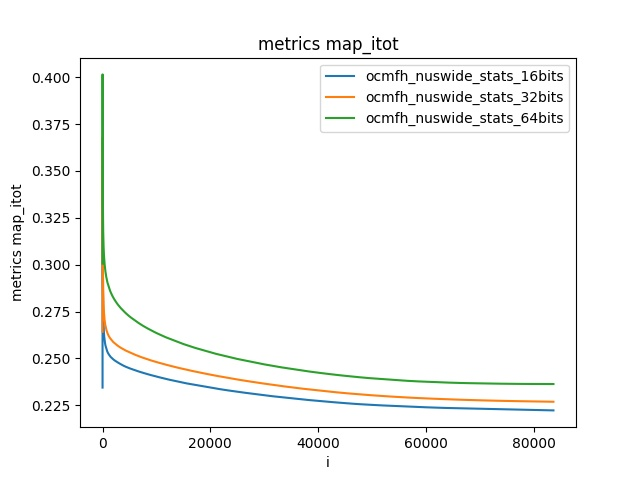
\includegraphics[width=\linewidth]{resultsImages/map/metrics map_itot_ocmfh_nuswide.jpeg}
                % \caption{Query type: min}
                % \label{fig:six_core_min}
                % \vspace{0.1ex}
                % \hspace{0ex}
            \end{minipage}
            \begin{minipage}[!h]{0.6\linewidth}
                \centering
                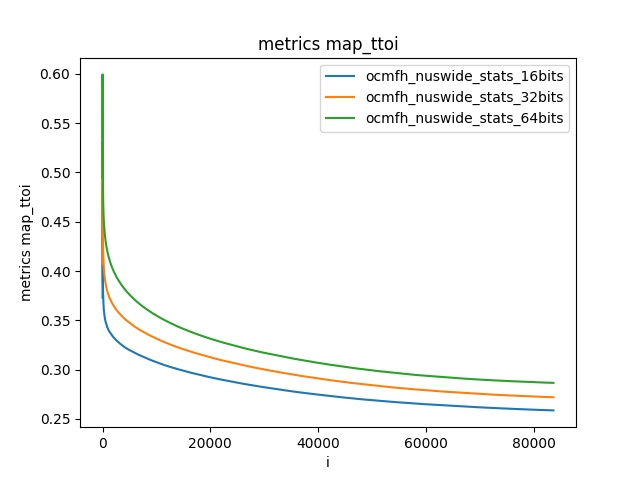
\includegraphics[width=\linewidth]{resultsImages/map/metrics map_ttoi_ocmfh_nuswide.jpeg}
                % \caption{Query type: sum}
                % \label{fig:six_core_sum}
                % \vspace{0.1ex}
                % \hspace{0ex}
            \end{minipage}
            \begin{minipage}[!h]{0.6\linewidth}
                \centering
                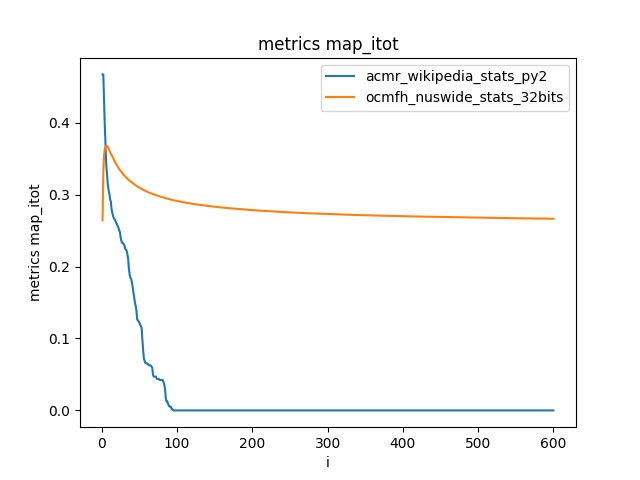
\includegraphics[width=\linewidth]{resultsImages/map/metrics map_itot_both_both.jpeg}
                % \caption{Query type: countrange}
                % \label{fig:six_core_countrange}
                % \vspace{0.1ex}
                % \hspace{0.1ex}
            \end{minipage}
            \begin{minipage}[!h]{0.6\linewidth}
                \centering
                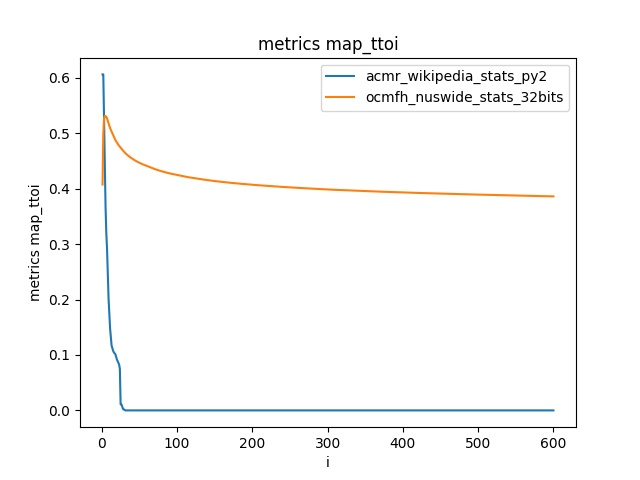
\includegraphics[width=\linewidth]{resultsImages/map/metrics map_ttoi_both_both.jpeg}
                % \caption{Query type: max}
                % \label{fig:six_core_max}
                % \vspace{0.1ex}
                % \hspace{0.1ex}
            \end{minipage}
        \caption{mAP metric for intra and inter method comparison on various datasets}
        \label{fig:}
        \end{figure}
        \FloatBarrier